\documentclass[14pt]{article}
\usepackage[french]{babel}
\usepackage[utf8]{inputenc}

\usepackage[T1]{fontenc}
\usepackage{textcomp}
\usepackage{amsfonts,amssymb}
\usepackage{amsmath}
\usepackage{pst-all}
\usepackage{graphicx}
\usepackage{float}
\usepackage{fancyhdr}
\usepackage{multicol}
\usepackage{pst-eucl}
\usepackage{pst-math}
\usepackage{chemfig}
\usepackage{tikz, tkz-tab}

%\usepackage{helvet}
%\usepackage{cmbright}

%\usepackage[lmargin=1cm,rmargin=1.5cm,vmargin={3cm,1cm},footskip={1.5cm}]{geometry}
\usepackage[left=1cm,right=1.2cm,top=2.3cm,bottom=2cm]{geometry}

% Tikz Libraries
\usetikzlibrary{calc,patterns,angles,quotes,optics,decorations.markings}

%\input{/home/edouard/maquereau/tabvar}





\newcommand{\N}{\mathbb N}
\newcommand{\Z}{\mathbb Z}
\newcommand{\Q}{\mathbb Q}
\newcommand{\K}{\mathbb K}
\newcommand{\R}{\mathbb R}
\newcommand{\C}{\mathbb C}
\newcommand{\U}{\mathbb U}
\newcommand{\PP}{\mathbb P}
\newcommand{\EE}{\mathbb E}
\newcommand{\VV}{\mathbb V}
%\newcommand{\vide}{\varnothing}

%\newcommand{\Acc}
%{\left\{\begin{array}}
%	\newcommand{\acC}
%	{\end{array}\right.}



\def\re{{\rm Re}\,}
\def\im{{\rm Im}\,}
\def\tn#1{\left|\left|\left|#1\right|\right|\right|}
\newcommand{\SN}[2]{[\! [{#1},{#2}]\! ]}% segment d'entiers
%Les lettres rondes
\def\A{\mathcal{A}}
\def\B{\mathcal{B}}
\def\Co{\mathcal{C}}
\def\Cl{\mathcal{C}}
\def\Cr{\mathcal{C}}
\def\Can{\mathcal{C}an}
\def\D{\mathcal{D}}
\def\E{\mathcal{E}}
\def\F{\mathcal{F}}
\def\G{\mathcal{G}}
\def\H{\mathcal{H}}
\def\I{\mathcal{I}}
\def\L{\mathcal{L}}
\def\M{\mathcal{M}}
\def\Nr{\mathcal{N}}
\def\P{\mathcal{P}}
\def\Qr{\mathcal{Q}}
\def\S{\mathcal{S}}
\def\T{\mathcal{T}}
\def\X{\mathcal{X}}
%\def\Rep{\mathcal{R}} %rep\`ere en g\'eom\'etrie affine
%\def\Inj{\mathcal{I}nj}
%\def\Bij{\mathcal{B}ij}
%\def\Esc{\mathcal{E}sc}
%\def\CM{\mathcal{CM}}
%\def\Gax{\mathcal{GA}}
\def\O{\mathcal{O}}

%\section{Masjuscules droites}
\mathcode`A="7041 \mathcode`B="7042 \mathcode`C="7043 \mathcode`D="7044
\mathcode`E="7045 \mathcode`F="7046 \mathcode`G="7047 \mathcode`H="7048
\mathcode`I="7049 \mathcode`J="704A \mathcode`K="704B \mathcode`L="704C
\mathcode`M="704D \mathcode`N="704E \mathcode`O="704F \mathcode`P="7050
\mathcode`Q="7051
\mathcode`R="7052
\mathcode`S="7053 \mathcode`T="7054
\mathcode`U="7055 \mathcode`V="7056 \mathcode`W="7057 \mathcode`X="7058
\mathcode`Y="7059 \mathcode`Z="705A

\newcommand{\dint}{\displaystyle\int}

\newcommand{\dsum}{\displaystyle\sum}




%d de l'int\'egrale
\def \d {\mathrm {d}}



%\newcommand{\der}[2]{\frac{\d#1}{\d#2}}% df/dx
%\newcommand{\Der}[2]{\dfrac{\d#1}{\d#2}}% df/dx en grand
%\newcommand{\dd}{\:\mathrm{d}}% d droit
%\newcommand{\diag}{\mathrm{diag}}% d droit
%\newcommand{\Dd}{\mathrm{D}}% D droit
%\newcommand{\drond}{\partial}% d rond
%\newcommand{\drp}[2]{\dfrac{\partial#1}{\partial#2}}% d\'eriv\'ees partielles
%\newcommand{\sdrp}[2]{\frac{\partial#1}{\partial#2}}% d\'eriv\'ees partielles
%\newcommand{\ddp}[2]{\dfrac{\partial^{2} #1}{\partial #2^{2}}}%derivee partielle 2
%\newcommand{\sddp}[2]{\tfrac{\partial^{2} #1}{\partial #2^{2}}}%
%small derivee partielle 2
%\newcommand{\dpp}[3]{\dfrac{\partial^{2} #1}{\partial #2 \partial #3}}%
%derivee partielle crois\'ees d'ordre 2



%DL
\def \o {\mathrm {o}}



%Les op\'erateurs

\DeclareMathOperator{\Max}{Max}
\DeclareMathOperator{\Min}{Min}

\DeclareMathOperator{\Sup}{Sup}
\DeclareMathOperator{\Inf}{Inf}
\DeclareMathOperator{\card}{card}
\newcommand{\Card}{\mathop{\mathrm{Card}}\nolimits}

%fonctions usuelles
\newcommand{\cl}[1]{\mathcal{C}^{#1}}% de classe ...
%\section{fonctions usuelles}
\newcommand{\Arctan}{\mathop{\mathrm{Arctan}}\nolimits}
\newcommand{\Arcsin}{\mathop{\mathrm{Arcsin}}\nolimits}
\newcommand{\Arccos}{\mathop{\mathrm{Arccos}}\nolimits}
\newcommand{\Argth}{\mathop{\mathrm{Arg\,th}}\nolimits}
\newcommand{\argth}{\mathop{\mathrm{Arg\,th}}\nolimits}
\newcommand{\Argsh}{\mathop{\mathrm{Arg\,sh}}\nolimits}
\newcommand{\argsh}{\mathop{\mathrm{Arg\,sh}}\nolimits}
\newcommand{\Argch}{\mathop{\mathrm{Arg\,ch}}\nolimits}
\newcommand{\argch}{\mathop{\mathrm{Arg\,ch}}\nolimits}
\newcommand{\ch}{\mathop{\mathrm{ch}}\nolimits}
\newcommand{\sh}{\mathop{\mathrm{sh}}\nolimits}
\renewcommand{\th}{\mathop{\mathrm{th}}\nolimits}
\newcommand{\J}{\mathop{\mathrm{j}}\nolimits}



\newcommand{\Tta}{\theta}
\newcommand{\tta}{\theta}

\newcommand{\LL}{{\cal L}}
\newcommand{\id}{{\rm Id}}
%\newcommand{\w}{{\cal W}}
%\newcommand{\V}{{\cal V}}
\newcommand{\e}{{\rm e}}
%\newcommand{\h}{{\cal H}}
\newcommand{\fy}{\varphi}
\newcommand{\ff}{{\cal F}}
%\newcommand{\so}{{\cal S}}
%\newcommand{\s}{\sigma}
%\newcommand{\te}{\theta}
%\newcommand{\LB}{{\cal LB}}
\newcommand{\ppq}{\leqslant}
\newcommand{\pgq}{\geqslant}
\newcommand{\al}{\alpha}
\newcommand{\eps}{\varepsilon}
%\newcommand{\ii}{{\rm I}}



%\catcode`\\'e=\active
%\def\'e{\'e}
%
%\catcode`\\`e=\active
%\def\`e{\`e}
%
%\catcode`\\^e=\active
%\def\^e{\^e}
%
%\catcode`\\`a=\active
%\def\`a{\`a}
%
%\catcode`\\^a=\active
%\def\^a{\^a}
%
%\catcode`\\`u=\active
%\def\`u{\`u}
%
%\catcode`\\^o=\active
%\def\^o{\^o}
%
%\catcode`\\^\i =\active
%\def\^\i {\^i}


%alg\`ebre lin\'eaire
%\DeclareMathOperator{\Ker}{Ker}
%\DeclareMathOperator{\Det}{Det}
%\DeclareMathOperator{\rg}{rg}
%\DeclareMathOperator{\Ima}{Im}
%\DeclareMathOperator{\vect}{vect}
%\DeclareMathOperator{\Id}{Id}
%\DeclareMathOperator{\Mat}{Mat}
%\DeclareMathOperator{\GL}{GL}
%\DeclareMathOperator{\SO}{SO}
%\newcommand{\Sp}{\mathop{\mathrm{Sp}}\nolimits} % spectre
\def \Tr {\mathrm{tr}}
%\newcommand{\trans}[1]{{\,}^{t} \! #1}

%Les nouvelles commandes

\def \i {\mathrm {i}}

\def\changemargin#1#2{\list{}{\rightmargin#2\leftmargin#1}\item[]}
\let\endchangemargin=\endlist


%\newcommand{\ens}[2]{\left\{#1 \,/\, #2\right\}}



%\newcommand{\ds}[3]{\displaystyle{\sum_{#1}^{#2}#3}}
%\newcommand{\dpr}[3]{\displaystyle{\prod_{#1}^{#2}#3}}

%\newcommand{\dl}[3]{\displaystyle{\lim_{#1 \rightarrow #2}#3}}


%\newcommand{\ve}[1]{\overrightarrow{#1}}
%\newcommand{\dintq}[4]{\displaystyle{\int_{#1}^{#2}{#3\,\d#4}}}

%\newcommand{\dintt}[3]{
%\displaystyle{\int_{#1}^{#2}{ #3}}}
%\newcommand{\dint}[2]{\displaystyle{\int{#1\,\d#2}}}






\pagestyle{fancy}

\lhead{\textbf{Amar AHMANE}}
\chead{\textbf{TP Numéro 17 – Chimie}}
\rhead{\textbf{07-02-2021}}

%\renewcommand{\headrulewidth}{1.5pt}
%\renewcommand{\headrulewidth}{0pt}

\cfoot{%\textbf{\thepage/3}
}


\rfoot{\textbf{\thepage/7}
}
\cfoot{%\textbf{\thepage/4}
}
\lfoot{%\textbf{\thepage/3}
}


%\newcounter{toto}
\begin{document}

  \newcommand{\OH}{[\text{OH}^-]}
  \newcommand{\CC}{[\text{C}_{\text{4}}\text{H}_{\text{8}}\text{O}_{\text{2}}]}
  \newcommand{\lH}{\lambda_{\text{OH}^-}}
  \newcommand{\lN}{\lambda_{\text{Na}^+}}
  \newcommand{\lC}{\lambda_{\text{C}_{\text{2}}\text{H}_{\text{3}}\text{O}_{\text{2}}^-}}

  \centerline{\textbf{Transformation de la matière.}}

  \centerline{Étude d'une cinétique par \textbf{conductimétrie.}}

  \centerline{Compte rendu du TP.}


  \begin{center}
    $\ast \ast \ast $
  \end{center}

  \begin{center}
		\textbf{\Large Introduction}
	\end{center}


	\vspace{4mm}

	\begin{center}
		\schemestart
			%\chemfig{*6(=-(-(-[1]*6(=-=-=-[::15]))-[-2])=-=(-N(-[2])-[::60])-)}
			\setchemfig{atom sep=2.5em}
			\small \chemfig{-[1](=[2]O)-[-1]O-[1]-[-1]}
		\schemestop\\
		\vspace{5mm}
		\textsc{Fig. 1} – Représentation plane de l'éthanoate d'éthyle.
	\end{center}

  Au cours du précédent TP, nous avons pu effectuer un suivi cinétique de la réaction du cristal violet avec les ions hydroxydes afin de déterminer l'ordre global de la réaction. Cette fois-ci, nous metterons en oeuvre une autre méthode expérimentale nous permettant de déterminer l'ordre globale d'une réaction. Il s'agit en l'occurence de la réaction de saponification de l'acétate d'éthyle (ou éthanoate d'éthyle), et le suivi se fera par \textbf{conductimétrie.}

  \begin{center}
		\schemestart
			CH$_3$CO$_2$C$_2$H$_5$ + OH$^{-}$
      \arrow{->}
      CH$_3$CO$_2$ $^{-}$ + C$_2$H$_5$OH
		\schemestop\\
		\vspace{5mm}
		\textsc{Éq. 1} – Équation de la réaction étudiée.
	\end{center}

  \begin{equation}
    \textit{La réaction est totale.}
  \end{equation}

  Nous réaliserons ainsi cette réaction et mesurerons la conductivité de la solution pour une durée de 20 minutes, le but étant, en connaissant la valeur de la conductivité initiale $\sigma_0$ et de la conductivité finale $\sigma_{\infty}$, de montrer que l'ordre global de cette réaction, puisqu'elle en admet un, est \textbf{2} et de déterminer, à la fin, l'énergie d'activation. Un travail préliminaire théorique nous permettra de mener à bien cette étude.

  \begin{center}
		\textbf{\Large Préliminaires}
	\end{center}

  Tout d'abord, la loi de vitesse de la réaction peut s'écrire :
  \[
    \boxed{v=k\times[\text{C}_{\text{4}}\text{H}_{\text{8}}\text{O}_{\text{2}}]^\alpha\times[\text{OH}^-]^\beta}
  \]
  où $k$ est la constante de vitesse, $\alpha$ et $\beta$ les ordres partiels. Or, les deux réactifs sont introduits en concentration égale, il s'ensuit que :
  \begin{equation}
    v=k\times\OH^{\alpha+\beta}
  \end{equation}


  On suppose à présente que $\alpha+\beta=2$. La loi de vitesse peut aussi s'écrire :
  \[
    v=-\frac{d\OH}{dt}
  \]
  Et on en déduit, d'après le relation (2), l'équation différentielle suivante :
  \[
    \frac{d\OH}{dt}=-k\times\OH^2
  \]
  En dissociant les variables et en intégrant entre $t_0$ et un temps quelconque $t$, on a :
  \[
    \int_{\OH_0}^{\OH_t}\frac{-d\OH}{\OH^2}=k\times\int_0^t\ dt
  \]

  \newpage

  Et il en résulte :
  \begin{equation}
    \boxed{\frac{1}{\OH_t}=kt+\frac{1}{\OH_0}}
  \end{equation}\\


  Et on pose $C_0=\OH=\CC$.


  Remarquons que $\frac{1}{\OH_t}=f(t)$ est une fonction affine de $t$.


  À présent, faisons une étude théorique de la réaction, notamment en nous intéressant à l'évolution de la conductivité en fonction du temps. D'après (1), la réaction est totale, ceci nous permet de dresser le tableau d'avancement suivant :
  \begin{center}
    \begin{tabular}{ | p{2cm} | c | c | c | c | }
      \hline
      & \chemfig{C_4H_8O_2} & \chemfig{OH}$^-$ & \chemfig{C_2H_3O_2}$^-$ & \chemfig{C_2H_6O}\\
      \hline
      $t=0$ & $C_0$ & $C_0$ & $0$ & $0$
      \\
      \hline
      $t$ & $C_0-x$ & $C_0-x$ & $x$ & $x$\\
      \hline
      $t=t_\infty$ & $0$ & $0$ & $C_0$ & $C_0$
      \\
      \hline
    \end{tabular}
  \end{center}

  Rappelons l'expression de la conductivité d'une solution, elle est égale à la somme des conductivités dues à chaque ion. Comme les espèces sont toutes monochargées, on a :
  \[
    \boxed{\sigma=\sum_i \lambda_i\times[X_i]}
  \]

  où \(\lambda_{i}\) est la conductivité molaire ionique de l'espèce \(X_{i}\). On note dans ce cas \(\sigma_{0}\) la conductivité à \(t=0\), \(\sigma\) la conductivité à un instant \(t\) quelconque, et enfin \(\sigma_{\infty}\) la conductivité de la solution à \(t_{\infty}\). Remarquons que $\sigma$ décroit au cours du temps : en effet, on assiste à une disparition d'ions hydroxydes et à une formation d'ions $\text{CH}_3\text{CO}_\text{2}^-$, or leur conductivité molaire ionique est inférieure à celle des ions $\text{OH}^-$; ainsi, la somme des conductivités décroît. On donne les expressions des grandeurs que nous venons de définir :
  \begin{gather}
    \begin{cases}
      \sigma_0= C_0\times \lH+C_0\times \lN\\
      \sigma = (C_0-x)\times \lH + x\times\lC+C_0\times \lN\\
      \sigma_\infty = C_0\times \lC+C_0\times \lN
    \end{cases}
  \end{gather}

  Il en découle :
  \[
    \frac{\sigma_0-\sigma_\infty}{\sigma-\sigma_\infty}=\frac{C_0(\lH-\lC)}{(C_0-x)(\lH-\lC)}=\frac{C_0}{C_0-x}
  \]

  Autrement dit :
  \begin{equation}
    \boxed{\frac{\sigma_0-\sigma_\infty}{\sigma-\sigma_\infty}=\frac{C_0}{\OH_t}}
  \end{equation}

  Ainsi, mesurer la conductivité de la solution au cours du temps nous permettra de tracer la droite $\frac{1}{\OH_t}=f(t)$ à une constante près. En effet, d'après (3) :
  \begin{equation}
    \frac{C_0}{\OH_t}=1+C_0kt
  \end{equation}



  \begin{center}
		\textbf{\Large Expérienc et résultats}
	\end{center}

  \vspace{4mm}

  On travaille à une température de $T_1=294,15$ K. Comme il est difficile de mesure la conductivité initiale après avoir lancé la réaction, on dilue $50$mL de soude à $0,05$mol.L$^{-1}$ dans $50$mL d'eau distillée, et on mesure $\sigma_0$ après agitation. De la même manière, pour ne pas attendre trop longtemps, on dilue $50$mL d'éthanoate de sodium à $0,05$mol.L$^{-1}$ dans $50$mL d'eau distillée, on mesure $\sigma_\infty$ après agitation.
  \begin{center}
    \begin{tabular}{| p{1.2cm} | p{3cm} |}
    \hline
    $\sigma_0$ & $4,94$mS.cm$^-1$\\
    \hline
    $\sigma_\infty$ & $1,0225$mS.cm$^-1$ \\
    \hline
    \end{tabular}
  \end{center}

  On verse ensuite $50$mL de soude à $0,05$mol.L$^{-1}$ dans un bécher de $150$mL, on y ajoute $50$mL d'éthanoate d'éthyle à $0,05$mol.L$^{-1}$; on déclanche le chronomètre dès que la totalité du volume a été versée. On note la conductivité de la solution chaque $30$s pendant 20 minutes. Le tableau de valeurs est disponible en annexe. \\

  \subsubsection*{Calculs numériques}
  Dans cette sous-partie, nous utiliserons un programme Python pour effectuer les calculs numériques. Nous reprenderons les fonctions du fichier \texttt{parser.py} qu'on a utilisées dans le précédent compte-rendu, que nous importerons dans un fichier que nous nommerons cette fois-ci \texttt{main.py}, le programme est toujours disponible en annexe. On trace alors $\frac{C_0}{\OH_t}$ en fonction de $t$, et on regarde les résultats qu'on obtient en console.
  \begin{center}
    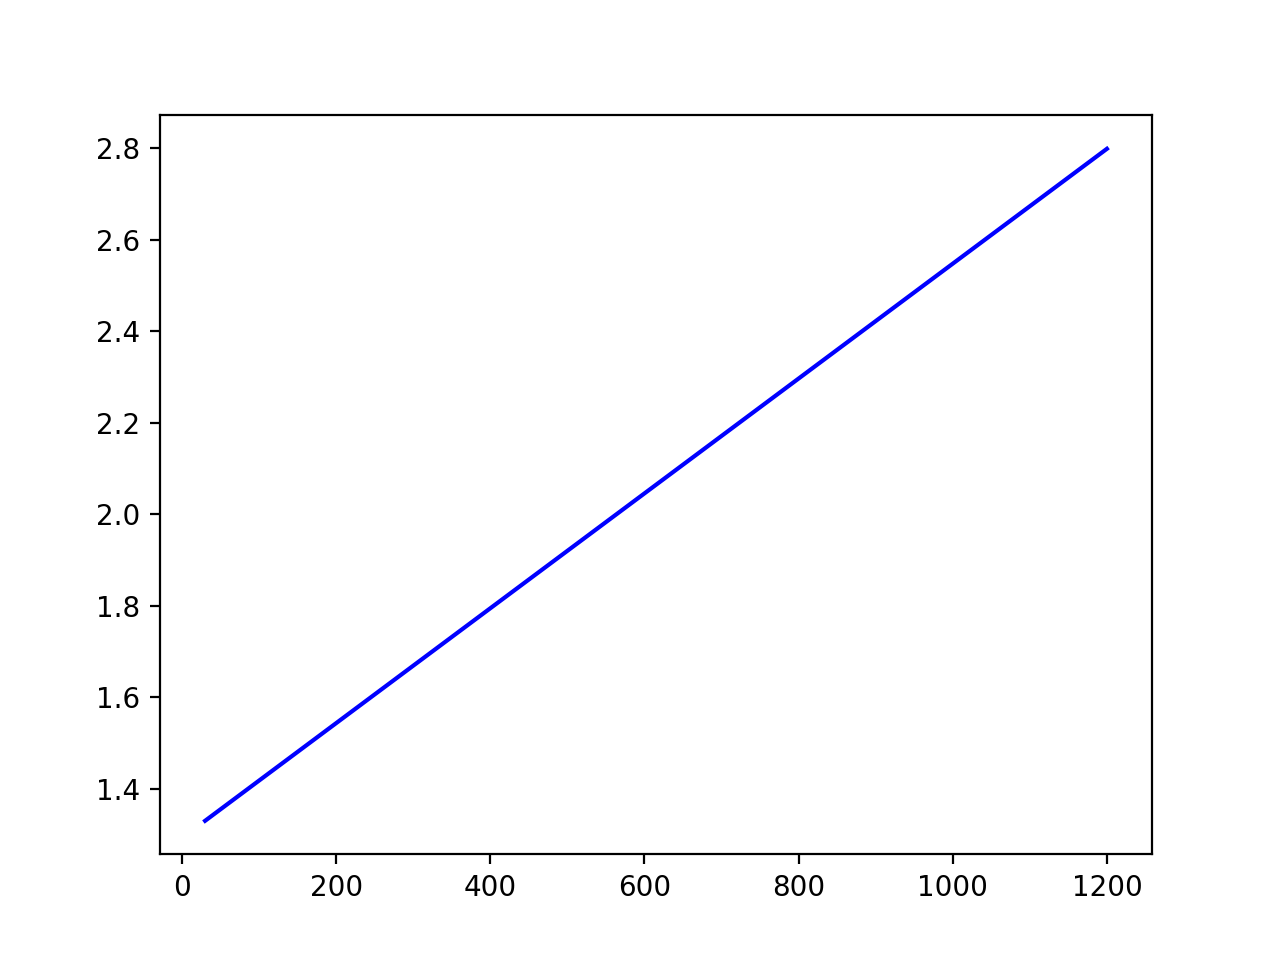
\includegraphics[scale=0.6]{./regg1.png}\\
    \textsc{Fig 2.} – $\frac{C_0}{\OH_t}=f(t)$
  \end{center}


  Les résultats en console donnent :
	\begin{changemargin}{1cm}{0mm}
		\noindent
		\texttt{tiplouf:cmeter mac\$ p3 main.py}\\
		\noindent
		\texttt{r**2 = 0.9907695417208003}\\
		\noindent
		\texttt{a = C0*k = [0.00125436] b = 1.293032827451996}\\
	\end{changemargin}

  L'ordre 2 est donc bien validé. De plus, le coefficient directeur étant $C_0\times k$, on peut en déduire la valeur de $k$, on a
  \begin{equation}
    k(T_1)=\frac{a}{C_0}=5,01744\times 10^{-2}\text{ L.mol}^{-1}\text{s}^{-1}
  \end{equation}


  En sachant qu'à $T_2=277,15$K, $k(T_2)=1,06\times 10^{-2}\text{ L.mol}^{-1}\text{s}^{-1}$, on peut en déduire l'énergie d'activation $E_a$. En effet, la loi d'Arrhenius permet d'établir :
  \begin{align*}
    \begin{cases}
      k(T_1)=A\times\exp\left(\frac{-E_a}{RT_1}\right)\\
      k(T_2)=A\times\exp\left(\frac{-E_a}{RT_2}\right)
    \end{cases} & \Leftrightarrow \frac{k(T_1)}{k(T_2)}=\exp\left(\frac{E_a}{RT_2}-\frac{E_a}{RT_1}\right)\\
    & \Leftrightarrow \ln\left(\frac{k(T_1)}{k(T_2)}\right)=E_a\times \left(\frac{1}{RT_2}-\frac{1}{RT_1}\right)\\
    & \Leftrightarrow E_a = \frac{RT_1T_2\ln\left(\frac{k(T_1)}{k(T_2)}\right)}{T_1-T_2}
  \end{align*}

  \paragraph{Application numérique : } $\boxed{E_a=61980.23\text{ J.mol}^{-1}}$

  \begin{center}
    $\ast \ast \ast $
  \end{center}

  \newpage

  \begin{center}
		\textbf{\Large Annexe}
	\end{center}

  \subsubsection*{Données : } Ci-dessous, le tableau contenant les valeurs de la conductivité mesurées à intervalles réguliers pendant 20 minutes.

  \begin{center}
  \begin{tabular}{|c|c|c|}
    \hline
    $i$ & $t$ & $\sigma$\\
    \hline
    & s & S/cm\\
    \hline\hline
    0 & 30,00 & 4,110\\
    1 & 60,00 & 4,010\\
    2 & 90,00 & 3,900\\
    3 & 120,0 & 3,800\\
    4 & 150,0 & 3,700\\
    5 & 180,0 & 3,630\\
    6 & 210,0 & 3,540\\
    7 & 240,0 & 3,480\\
    8 & 270,0 & 3,410\\
    9 & 300,0 & 3,350\\
    10 & 330,0 & 3,290\\
    11 & 360,0 & 3,240\\
    12 & 390,0 & 3,190\\
    13 & 420,0 & 3,140\\
    14 & 450,0 & 3,100\\
    15 & 480,0 & 3,060\\
    16 & 510,0 & 3,020\\
    17 & 540,0 & 2,980\\
    18 & 570,0 & 2,950\\
    19 & 600,0 & 2,920\\
    \hline
  \end{tabular}
  \begin{tabular}{|c|c|c|}
    \hline
    $i$ & $t$ & $\sigma$\\
    \hline
    & s & S/cm\\
    \hline\hline
    20 & 630,0 & 2,890\\
    21 & 660,0 & 2,860\\
    22 & 690,0 & 2,830\\
    23 & 720,0 & 2,810\\
    24 & 750,0 & 2,780\\
    25 & 780,0 & 2,760\\
    26 & 800,0 & 2,680\\
    27 & 810,0 & 2,740\\
    28 & 830,0 & 2,660\\
    29 & 840,0 & 2,710\\
    30 & 860,0 & 2,640\\
    31 & 870,0 & 2,700\\
    32 & 890,0 & 2,620\\
    33 & 920,0 & 2,610\\
    34 & 950,0 & 2,590\\
    35 & 980,0 & 2,580\\
    36 & 1010 & 2,560\\
    37 & 1040 & 2,550\\
    38 & 1070 & 2,512\\
    39 & 1200 & 2,502\\
    \hline
  \end{tabular}
  \end{center}

  \subsubsection*{Programme informatique}

  Voici le fichier \texttt{main.py}
	\begin{center}
		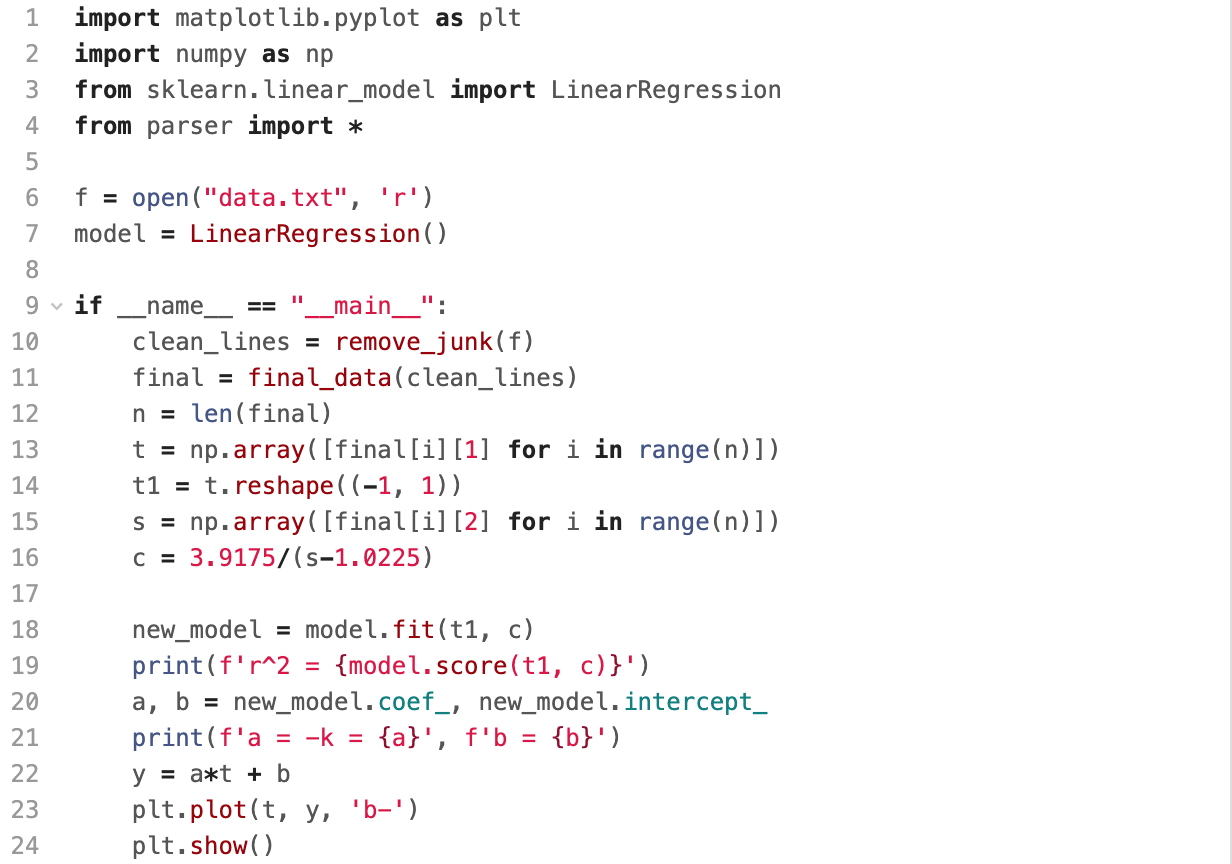
\includegraphics[scale=0.5]{./01.png}
	\end{center}

\end{document}
